\documentclass[10pt,a4paper]{article}
\usepackage{ctex}
\usepackage{fancyhdr}
\usepackage{booktabs}
\usepackage{graphicx}
\usepackage{amsmath}
\usepackage{float}
\usepackage{xcolor}
\usepackage{listings}
\usepackage{multirow}
\usepackage{diagbox}
\usepackage[table]{xcolor}
\usepackage{subcaption}
\usepackage[colorlinks,linkcolor=blue]{hyperref} % 用于插入超链接

% 文章页面margin设置
\usepackage[a4paper]{geometry}
\geometry{top=1in}
\geometry{bottom=1in}
\geometry{left=0.75in}
\geometry{right=0.75in}   % 设置上下左右页边距
\geometry{marginparwidth=1.75cm}    % 设置边注距离(注释、标记等)

% 设置页眉
\pagestyle{fancy}
\fancyhf{}
\lhead{《人工智能基础》课程实验报告}
\chead{王荦璠,朱首赫}
\rhead{\thepage}
\renewcommand{\headrulewidth}{0.4pt}

% 代码设置
\lstset{
    basicstyle=\ttfamily\small,
    numbers=left,
    numberstyle=\tiny,
    keywordstyle=\color{blue},
    commentstyle=\color{green!60!black},
    stringstyle=\color{red},
    breaklines=true,
    frame=single,
    showstringspaces=false
}

\begin{document}

\begin{center}
    \LARGE{\textbf{个性化新闻标题生成:PENS基线方法改进与提示词工程方法的实现}}
    
    \vspace{0.5cm}
    \large{王荦璠,朱首赫}
    
    \vspace{0.3cm}
    \today
\end{center}

\section{完成情况概述}
本组选择的课题为“个性化标题生成任务”,通过搭建github仓库进行协作开发,目前已完成了两个备选技术路线,包括PENS基线方法复现与改进、基于提示工程的大模型个性化生成方法。现有可运行的完整代码和清晰的Readme文档,及自行设计的创新评估方案。

\section{PENS基线方法复现与改进}
\subsection{环境搭建}
本地环境已配置 CUDA 11.8,以满足深度学习任务中对 GPU 加速的需求。考虑到项目涉及多种深度学习库(包括 PyTorch、Transformers、NumPy 等),为保障依赖管理的稳定性与可复现性,采用 Conda 作为环境管理工具,并依据基线项目提供的 requirements.txt 文件构建了独立的虚拟环境。。

\subsection{基线方法分析}
\subsubsection{整体架构}
项目遵循一个经典的三阶段流水线架构:数据预处理 (Preprocess) -> 用户建模 (UserEncoder) -> 个性化生成 (Generator)。开始时,原始数据存储在 'data/' 目录中,首先需要'Preprocess' 组件将原始数据清洗、转换并结构化,输出到 'data2/' 目录,这个目录下的数据是后续所有模型训练的直接数据源。然后'UserEncoder' 和 'Generator' 组件分别进行模型训练,并将训练好的模型(即组件的产物)保存在 'runs/' 目录下的相应子目录中。这个过程中,下游组件明确依赖上游组件的产物:'UserEncoder' 依赖 'data2/' 的数据,而 'Generator' 则同时依赖 'data2/' 的数据和 'UserEncoder' 训练出的模型。
\subsubsection{核心组件分析}
\textbf{数据预处理 (Preprocess):}在 PENS 个性化新闻标题生成项目中,数据预处理(Preprocess)组件是整个工作流的起点,其核心逻辑集中在 pensmodule/Preprocess/preprocess.ipynb 中。该组件的主要职责是将原始的、非结构化的新闻文本和用户行为日志转化为深度学习模型可接受的标准化数值格式。其内部由多个功能模块组成,虽非独立 Python 脚本,但通过 Jupyter Notebook 的代码单元顺序执行形成了完整的流水线。首先,环境配置模块导入必要的库(如 pandas、numpy、nltk、torch)并定义全局超参数(如 MAX\_CONTENT\_LEN, WORD\_FREQ\_THRESHOLD 等),为数据处理流程设定统一标准。接着,新闻解析模块(read\_news)读取原始 news.tsv 文件,执行文本清洗、分词、词频统计,并构建 word\_dict、category\_dict、news\_index 等核心词典映射。随后,这些词典和索引信息被序列化保存至\\data2目录下(如图\ref{fig:processed_data}),作为项目中的首个数据检查点。为满足下游模型输入格式,Preprocess 分别为用户编码器(UserEncoder)和标题生成器(Generator)生成不同的数据表示。前者生成固定长度的新闻标题、正文和类别 ID 序列并保存为 .npy 文件,后者则构建 Seq2Seq 模型所需的源-目标对,包含正文输入、标题输入与输出序列。此外,组件还通过加载预训练 GloVe 向量为项目构建词嵌入矩阵,并处理用户点击日志,生成用户点击历史和训练样本,包括正负样本配对。最终,这些用户数据也被序列化存储,成为后续模型训练的基础。整个 Preprocess 组件通过内存变量传递与文件系统持久化相结合的方式,确保数据处理的连续性、结构的清晰性和下游可复用性,是实现项目个性化生成能力的坚实数据基础。

\begin{figure}[H]
  \centering
  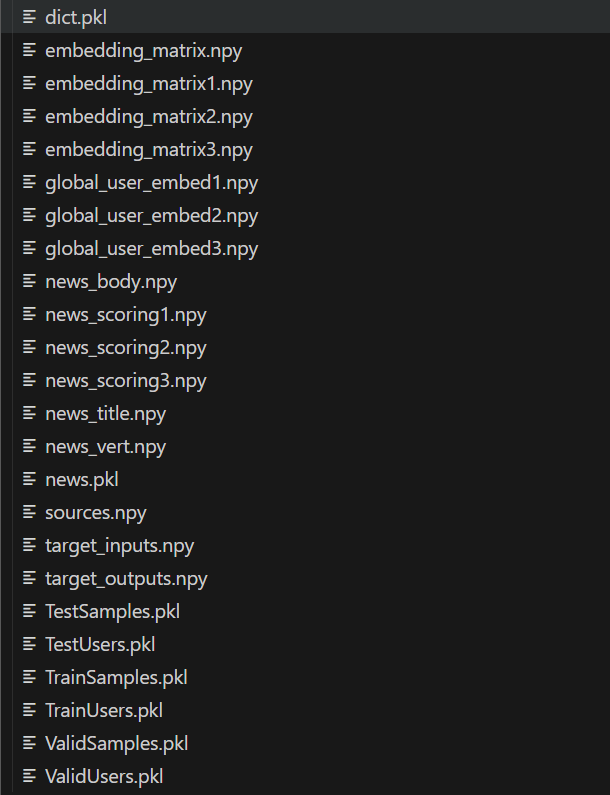
\includegraphics[width=10cm]{fig/processed_data.png}
  \caption{预处理后的数据}\label{fig:processed_data}
\end{figure}


\textbf{用户编码器(UserEncoder):}
该组件承担着"理解用户"的核心职责,其目标是将用户的历史点击行为转化为一个固定维度的用户兴趣向量(User Vector),用于指导下游的标题生成模型。该组件以 Preprocess 组件生成的结构化数据为输入,最终输出一个训练好的深度学习模型,逻辑分布于多个 Python 文件中,并由 Jupyter Notebook(pipeline\_Train\_Test.ipynb)协调执行。其工作流程首先由 data.py 负责数据加载,它将 .npy 和 .pkl 文件构造成可供 PyTorch 使用的 Dataset 和 DataLoader,其中每个训练样本包括候选新闻、用户点击历史及其标签。随后,modules.py 定义了多头注意力(MultiHeadAttention)和注意力池化(AttentionPooling)等通用网络结构,为 model.py 中的核心模型(如 NRMS)提供构建模块。model.py 则定义了新闻编码器和用户编码器的具体结构,利用词嵌入初始化、注意力机制等方法提取用户兴趣表示。辅助模块 utils.py 提供模型训练过程中的准确率评估函数,而训练的总流程则集中在 pipeline\_Train\_Test.ipynb 中,包括环境配置、数据加载、模型初始化、迭代训练、性能评估与模型保存。整个 UserEncoder 
组件高度模块化,逻辑清晰,其训练产物保存在 runs/userencoder/ 目录下(如图\ref{fig:user_encode}),并作为下游 Generator 组件生成个性化标题的重要输入。这种分工明确、耦合度低的设计使得组件易于维护、调试与替换。

\begin{figure}[H]
  \centering
  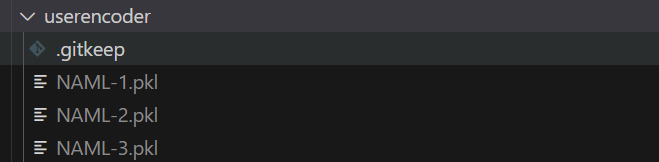
\includegraphics[width=10cm]{fig/user_encode.png}
  \caption{编码器输出}\label{fig:user_encode}
\end{figure}

\textbf{个性化生成器(Generator):}
该组件是整个系统的最终执行单元,其主要任务是融合来自 Preprocess 的结构化数据与 UserEncoder 提供的用户兴趣向量,生成既符合新闻内容又契合用户偏好的个性化新闻标题。该组件采用现代自然语言生成任务中经典的"预训练-微调"两阶段策略,由多个功能模块组成并通过 pipeline\_pretrain\_train\_test.ipynb 统一调度。首先,配置文件 config.json 提供了模型结构与训练超参数的全局定义;数据加载模块 data.py 负责将结构化数据转化为适用于训练的 PyTorch Dataset,其中 Seq2SeqDataset 用于通用预训练,ImpressionDataset 则加载用户点击历史与新闻向量用于个性化微调。模型的底层构件分布于 encoder.py、decoder\_pointer.py 与 modules.py 中,分别定义了编码器、带指针机制的解码器以及通用注意力层,实现了输入新闻文本的有效表示与个性化控制能力。model.py 中的 HeadlineGen 类则将上述模块整合为一个可训练的完整模型,其 forward 函数实现了对新闻文本的编码、结合用户兴趣向量解码生成标题的全过程。训练逻辑由 train.py 和 eval.py 等模块提供支持,封装了优化器、损失函数、微调逻辑、性能评估与 Beam Search 生成策略。整个训练与评估过程在 Jupyter Notebook 中有序展开:首先利用 Seq2SeqDataset 进行预训练,学习一般性标题生成能力;随后加载训练好的 UserEncoder 模型进行微调,将用户兴趣向量注入生成流程,从而实现真正的个性化生成,并将最终模型保存在 runs/ 目录(如图\ref{fig:model_weight})。

\begin{figure}[H]
  \centering
  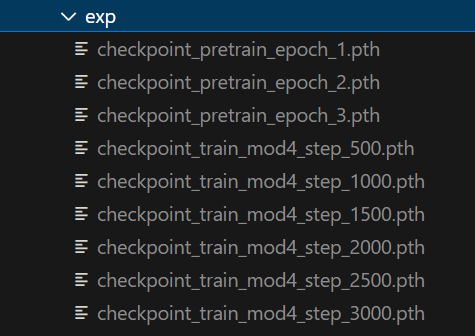
\includegraphics[width=10cm]{fig/model_weight.png}
  \caption{训练好的模型权重}\label{fig:model_weight}
\end{figure}

\subsection{基线方法改进}
\textbf{解决原代码的兼容性问题:}
在适配项目代码至 PyTorch 2.0 及以上版本时,发现原有模型加载方式存在兼容性问题。具体来说,原始代码在加载训练好的模型检查点时,直接使用 torch.load(checkpoint\_path)进行模型还原。但在 PyTorch 2.0 起,torch.load() 新增了一个默认参数 weights\_only=True,即默认仅加载模型的权重部分,而不恢复模型对象本身的结构。由于原代码并未显式指定 weights\_only=False,这会导致模型加载过程中,checkpoint['model'] 返回为 None 或空字典,从而在后续尝试调用模型属性、执行推理或微调操作时触发报错。因此,为保证代码的稳定运行与模型的完整还原,需要显式地在加载检查点时传入 weights\_only=False 参数(如下图\ref{fig:model_loader}),以确保模型结构与权重一并加载。此修复对于后续模块(如个性化生成器中的微调与推理)能否正常运行至关重要。

\begin{figure}[H]
  \centering
  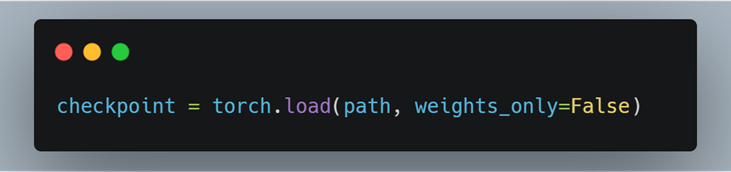
\includegraphics[width=10cm]{fig/load_new.png}
  \caption{改进后的模型加载方式}\label{fig:model_loader}
\end{figure}

\textbf{训练方法优化:}
在复现并运行原始项目训练流程(包括 UserEncoder 训练和 Generator 的预训练/微调)时,观察到本地 GPU 使用率严重不达标,训练过程中 GPU 占用率多数时间低于 10\%,功率也接近空闲状态,仅在个别时间段出现短暂上升,但峰值也较低。这种"GPU 闲置"现象表明,训练瓶颈不在模型计算,而是数据传输过程。通过分析数据加载过程发现,原始的 DataLoader 使用的是单线程加载策略,且未启用任何内存加速机制,导致 CPU 数据准备速度无法匹配 GPU 运算速度,从而频繁阻塞 GPU 等待输入。为此,笔者对训练数据加载流程进行了两项优化(如下图\ref{fig:data_loader}):其一是设置 DataLoader 的 num\_workers 参数为系统支持的较大值(如 20),启用多线程数据加载,提升数据读取与预处理速度;其二是启用 pin\_memory=True,将数据加载到固定内存(Pinned Memory),加快 CPU 到 GPU 的数据传输速度。这一系列改进显著提升了系统吞吐能力,使 GPU 占用率长期维持在 97\%~100\%,整体训练效率提高了约一倍,尤其在数据预处理、模型预训练和个性化微调阶段的迭代速度有了显著提升。

\begin{figure}[H]
  \centering
  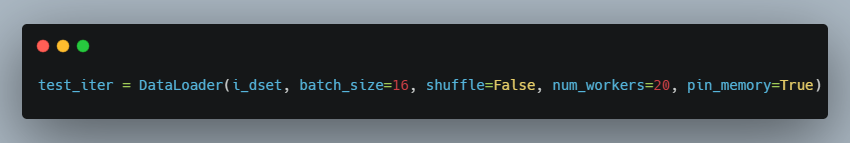
\includegraphics[width=15cm]{fig/dataloader.png}
  \caption{改进后的数据加载方式}\label{fig:data_loader}
\end{figure}


\textbf{新增功能模块:}
为提升项目的可用性与交互性,新增了一个名为 predict\_with\_trained\_model.ipynb 的功能模块,用于实现模型的推理应用与结果输出。该模块允许用户在训练完成后,直接加载训练好的个性化标题生成模型,并对指定输入数据(可以是原始新闻正文,也可以是用户自定义文本)执行标题生成任务。生成结果会自动保存在当前目录下的 generated\_titles.txt 文件中,便于查阅与后续分析。此外,如果用户同时提供了对应的"参考标题"(即人工撰写或已有的真实标题),系统还会自动调用内置的评估函数对生成结果进行 ROUGE 指标评分,量化模型的生成质量。该模块的添加不仅提升了项目的实用性,也为实际部署、用户交互和性能评估提供了便利。

\subsection{实验结果}
在完成对基线方法的完整复现后,我们对模型在不同训练阶段的性能表现进行了系统评估,相关实验结果已保存在 /docs0 目录下。主要评估指标包括训练过程中模型获得的奖励值(如图 \ref{fig:reward} 所示)和在验证集上的 ROUGE 指标得分变化(如图 \ref{fig:rouge} 所示)。图 \ref{fig:reward} 展示了在训练过程中的奖励曲线,可以观察到模型在初期训练阶段奖励提升较快,随后逐渐趋于平稳;图 \ref{fig:rouge} 则反映了模型生成结果在不同训练步数下与参考标题的相似度趋势。

从实验结果来看,若以 ROUGE 分数作为唯一的性能评价标准,可以明确观察到模型在训练至第 2000 步左右时达到了最佳表现,此时的 ROUGE-1、ROUGE-2 和 ROUGE-L 得分均达到当前训练流程下的峰值,表明模型在该阶段生成的标题在内容覆盖率、信息完整性以及语言结构上最为接近人工参考标题。

\begin{figure}[H]
  \centering
  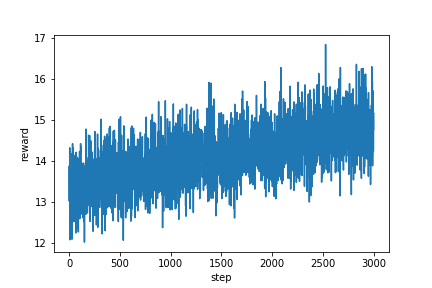
\includegraphics[width=10cm]{fig/reward.png}
  \caption{训练奖励随训练步数的变化}\label{fig:reward}
\end{figure}

\begin{figure}[H]
  \centering
  \begin{subfigure}{0.3\textwidth}
    \centering
    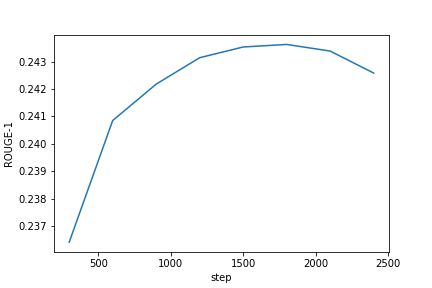
\includegraphics[width=\textwidth]{fig/rouge1.png}
  \end{subfigure}
  \hfill
  \begin{subfigure}{0.3\textwidth}
    \centering
    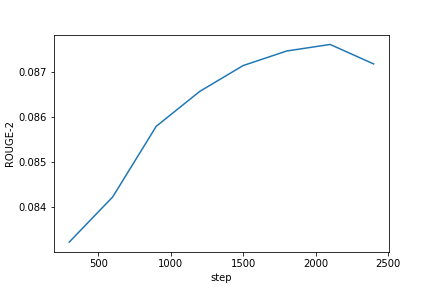
\includegraphics[width=\textwidth]{fig/rouge2.png}
  \end{subfigure}
  \hfill
  \begin{subfigure}{0.3\textwidth}
    \centering
    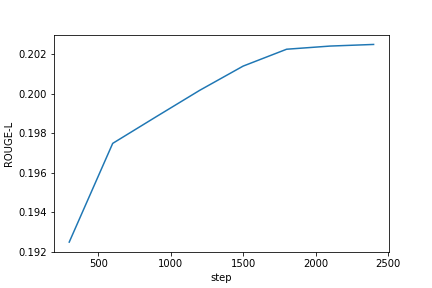
\includegraphics[width=\textwidth]{fig/rougel.png}
  \end{subfigure}
  \caption{ROUGE评分随训练步数的变化}\label{fig:rouge}
\end{figure}

此外,为进一步验证模型在真实应用场景下的生成能力,本项目调用已训练完成的个性化标题生成模型,对一组自定义新闻样本数据进行实验,生成了具有用户偏好的新闻标题。实验过程中,输入数据包含自定义的新闻正文内容,与之相关联的用户点击历史信息则沿用了原来的数据,模型基于这些信息综合判断用户兴趣,并在保证标题语义合理的基础上,生成更符合用户阅读偏好的标题文本。

图 \ref{fig:ref} 展示了该组自定义新闻样本所对应的人工参考标题;图 \ref{fig:gen} 展示了模型在上述输入条件下生成的个性化标题结果。通过对比可发现,生成标题1在覆盖新闻关键信息的同时,也在表达方式和用词选择上体现出一定的用户偏好倾向,例如更具吸引力的措辞、更符合用户点击倾向的词语顺序等。但标题2、3则表现不佳,不仅没有使用更吸引人的措辞,甚至丢失了原有新闻标题中的关键信息。可见该模型的可泛化性和实用性仍有待加强
。
\begin{figure}[H]
  \centering
  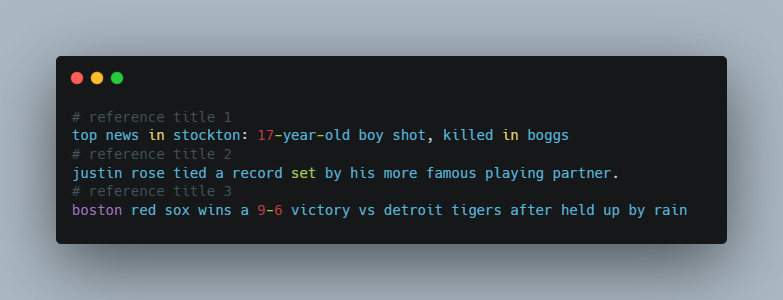
\includegraphics[width=15cm]{fig/reference.png}
  \caption{参考标题}\label{fig:ref}
\end{figure}
\begin{figure}[H]
  \centering
  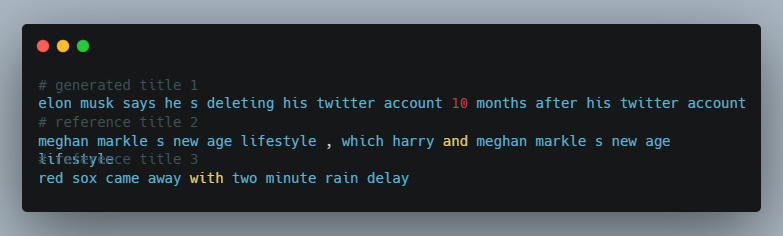
\includegraphics[width=15cm]{fig/generated.png}
  \caption{生成标题}\label{fig:gen}
\end{figure}


\section{基于提示词工程的个性化标题生成方法}
\subsection{中转API平台搭建}
为实现对大语言模型API的统一管理和高效调用,本项目在现有开源项目One-API和DeepClaude的基础上,通过自建服务器构建了ChavAPI中转平台(\url{https://api.chavapa.com})。该平台的搭建为提示词工程方法提供了坚实的技术支撑。

ChavAPI平台采用分布式架构设计,通过Docker容器化部署实现高可用性。平台核心功能包括:多模型统一接口封装、智能负载均衡、请求限流与配额管理、实时监控与日志记录等。在API密钥管理方面,平台支持多渠道密钥轮询使用,有效分散请求压力,并通过加密存储确保密钥安全。负载均衡策略方面,系统根据各API提供商的响应时间、成功率等指标动态调整请求分配,确保服务稳定性。同时,平台提供详细的用量统计和成本分析功能,支持按项目、按用户的精确计费,为本项目的预算控制提供了有力保障。

此外,ChavAPI平台在兼容性设计上严格遵循OpenAI API标准,使得项目代码能够无缝对接不同的大语言模型服务商,包括DeepSeek、GPT系列、Claude系列等主流模型。这种统一的接口设计不仅简化了代码开发流程,也为后续可能的模型横向对比实验提供了便利。

\subsection{本地环境搭建}
提示词工程方法的环境配置相对简洁,主要依赖Python生态系统和云端API服务。本地环境搭建包括Python 3.8+运行时、核心依赖包安装(OpenAI、Pandas、NumPy、Rouge-Score、Matplotlib等),以及Jupyter Notebook开发环境配置。与基线方法相比,该方案无需复杂的深度学习环境配置,避免了CUDA版本兼容、GPU显存管理等技术难题。

API配置管理采用模板化设计,通过\texttt{api\_config\_template.py}提供标准配置模板,用户仅需复制为\texttt{api\_config.py}并填入相应API密钥即可完成配置。配置文件支持多模型参数定义,包括推理模型(如DeepSeek-R1系列)和对话模型(如DeepSeek-Chat系列)的差异化设置。系统根据模型类型自动调整最大token数、温度参数等关键配置,确保不同模型的最优性能表现。

项目采用模块化的目录结构设计,核心组件包括数据处理器(\texttt{data\_processor.py})、提示词生成器(\texttt{prompt\_generator.py})、LLM客户端(\texttt{llm\_client.py})、评估器(\texttt{evaluator.py})等,各模块职责清晰,便于维护和扩展。输出目录按功能分类组织,包括预处理数据、生成标题、评估结果等子目录,确保实验数据的有序管理。

\subsection{提示词工程方法分析}
\subsubsection{整体架构}
提示词工程方法采用“数据驱动+智能提示”的技术路线,整体架构可分为四个核心阶段:数据预处理与用户画像构建、自适应提示词生成、大模型API调用与内容生成、多维度智能评估。与传统深度学习方法不同,该架构充分利用大语言模型的语言理解和生成能力,通过精心设计的提示词模板实现个性化内容生成,避免了复杂的模型训练过程。

系统工作流程如下:首先,数据处理器从原始PENS数据集中提取用户历史点击序列,通过统计分析构建用户兴趣档案,包括主要兴趣类别、偏好权重等信息;随后,提示词生成器根据目标新闻内容和用户画像,动态构建个性化的提示词模板;接着,LLM客户端调用大语言模型API,基于生成的提示词产出个性化标题;最后,评估器采用ROUGE自动评估、LLM智能评估等多种方法对生成结果进行综合评价。

\subsubsection{核心组件分析}
\textbf{数据预处理模块(DataProcessor):}该模块负责从原始TSV格式数据中提取用户行为序列和新闻内容,构建适用于提示词工程的结构化数据。核心功能包括用户历史点击序列提取、兴趣类别统计分析、测试样本准备等。与基线方法中的复杂特征工程不同,该模块专注于语义信息的保留和组织,将原始文本数据转化为易于理解的自然语言描述。用户兴趣提取算法通过分析点击历史中的新闻类别分布,计算各类别的点击频次和权重,确定用户的主要兴趣领域。数据处理过程中,系统会对新闻正文进行长度截断(限制在400字符以内),确保提示词总长度控制在模型的上下文窗口范围内。

\textbf{提示词生成器(PromptGenerator):}作为系统的核心组件,该模块实现了自适应的提示词生成策略,根据不同的模型类型(推理模型vs对话模型)和任务风格(聚焦式vs增强式vs创意式)动态选择最优的提示词模板。模块内部定义了分层的提示词结构,包括系统级提示词(定义任务目标和输出规范)和用户级提示词(包含具体的新闻内容和用户信息)。以下是系统提示词的核心片段:

\begin{lstlisting}[language=Python, caption=系统提示词示例]
system_prompt = """You are an AI expert at creating personalized news headlines. 
Your task is to analyze user preferences and generate engaging, personalized 
English headlines that match their interests.

Key requirements:
- Generate ONLY English headlines (no Chinese)
- Headlines should be 8-20 words long
- Make headlines personally relevant to the user's interests
- Maintain accuracy to the original news content
- Use engaging, attention-grabbing language
- Return ONLY the final headline text, no explanations"""
\end{lstlisting}

用户提示词模板则通过Python字符串格式化技术,将用户历史阅读记录、兴趣标签、原始新闻内容等信息有机融合,形成完整的生成指令。系统支持三种风格的提示词:聚焦式(简洁明了)、增强式(详细分析)、创意式(强调个性化表达),不同风格适用于不同的应用场景和模型特性。

\textbf{LLM客户端(LLMClient):}该模块封装了与大语言模型API的交互逻辑,支持多模型动态切换和自适应参数调整。客户端实现了智能的内容提取策略,能够处理推理模型和对话模型在响应格式上的差异。对于推理模型,系统会从reasoning字段中提取最终的标题内容;对于对话模型,则直接从content字段获取结果。模块还包含了完善的错误处理和重试机制,确保API调用的稳定性。以下代码展示了自适应内容提取的核心逻辑:

\begin{lstlisting}[language=Python, caption=自适应内容提取]
def _extract_content_adaptive(self, response):
    message = response.choices[0].message
    
    if self.is_reasoning_model:
        # 推理模型:优先检查content字段是否有效
        if message.content and message.content.strip():
            content = message.content.strip()
            if self._is_valid_title_content(content):
                return self.clean_generated_title(content)
        
        # 如果content无效,尝试从reasoning字段提取
        if hasattr(message, 'model_extra') and 'reasoning' in message.model_extra:
            reasoning = message.model_extra['reasoning']
            return self.extract_title_from_reasoning(reasoning)
    else:
        # 对话模型:直接使用content字段
        if message.content and message.content.strip():
            return self.clean_generated_title(message.content.strip())
\end{lstlisting}

\textbf{评估模块(Evaluator):}该模块实现了多维度的评估体系,结合传统的ROUGE自动评估和基于LLM的智能评估,全面衡量生成标题的质量和个性化效果。ROUGE评估计算生成标题与参考标题之间的词汇重叠度,包括ROUGE-1、ROUGE-2、ROUGE-L等指标。LLM智能评估则调用大语言模型对标题质量进行人工智能评分,评估维度包括准确性、吸引力、清晰度、合理性、创新性等。个性化效果评估采用规则引擎和LLM评估相结合的方式,从兴趣匹配度、类别相关性、历史一致性等角度量化个性化程度。

\begin{figure}[H]
  \centering
  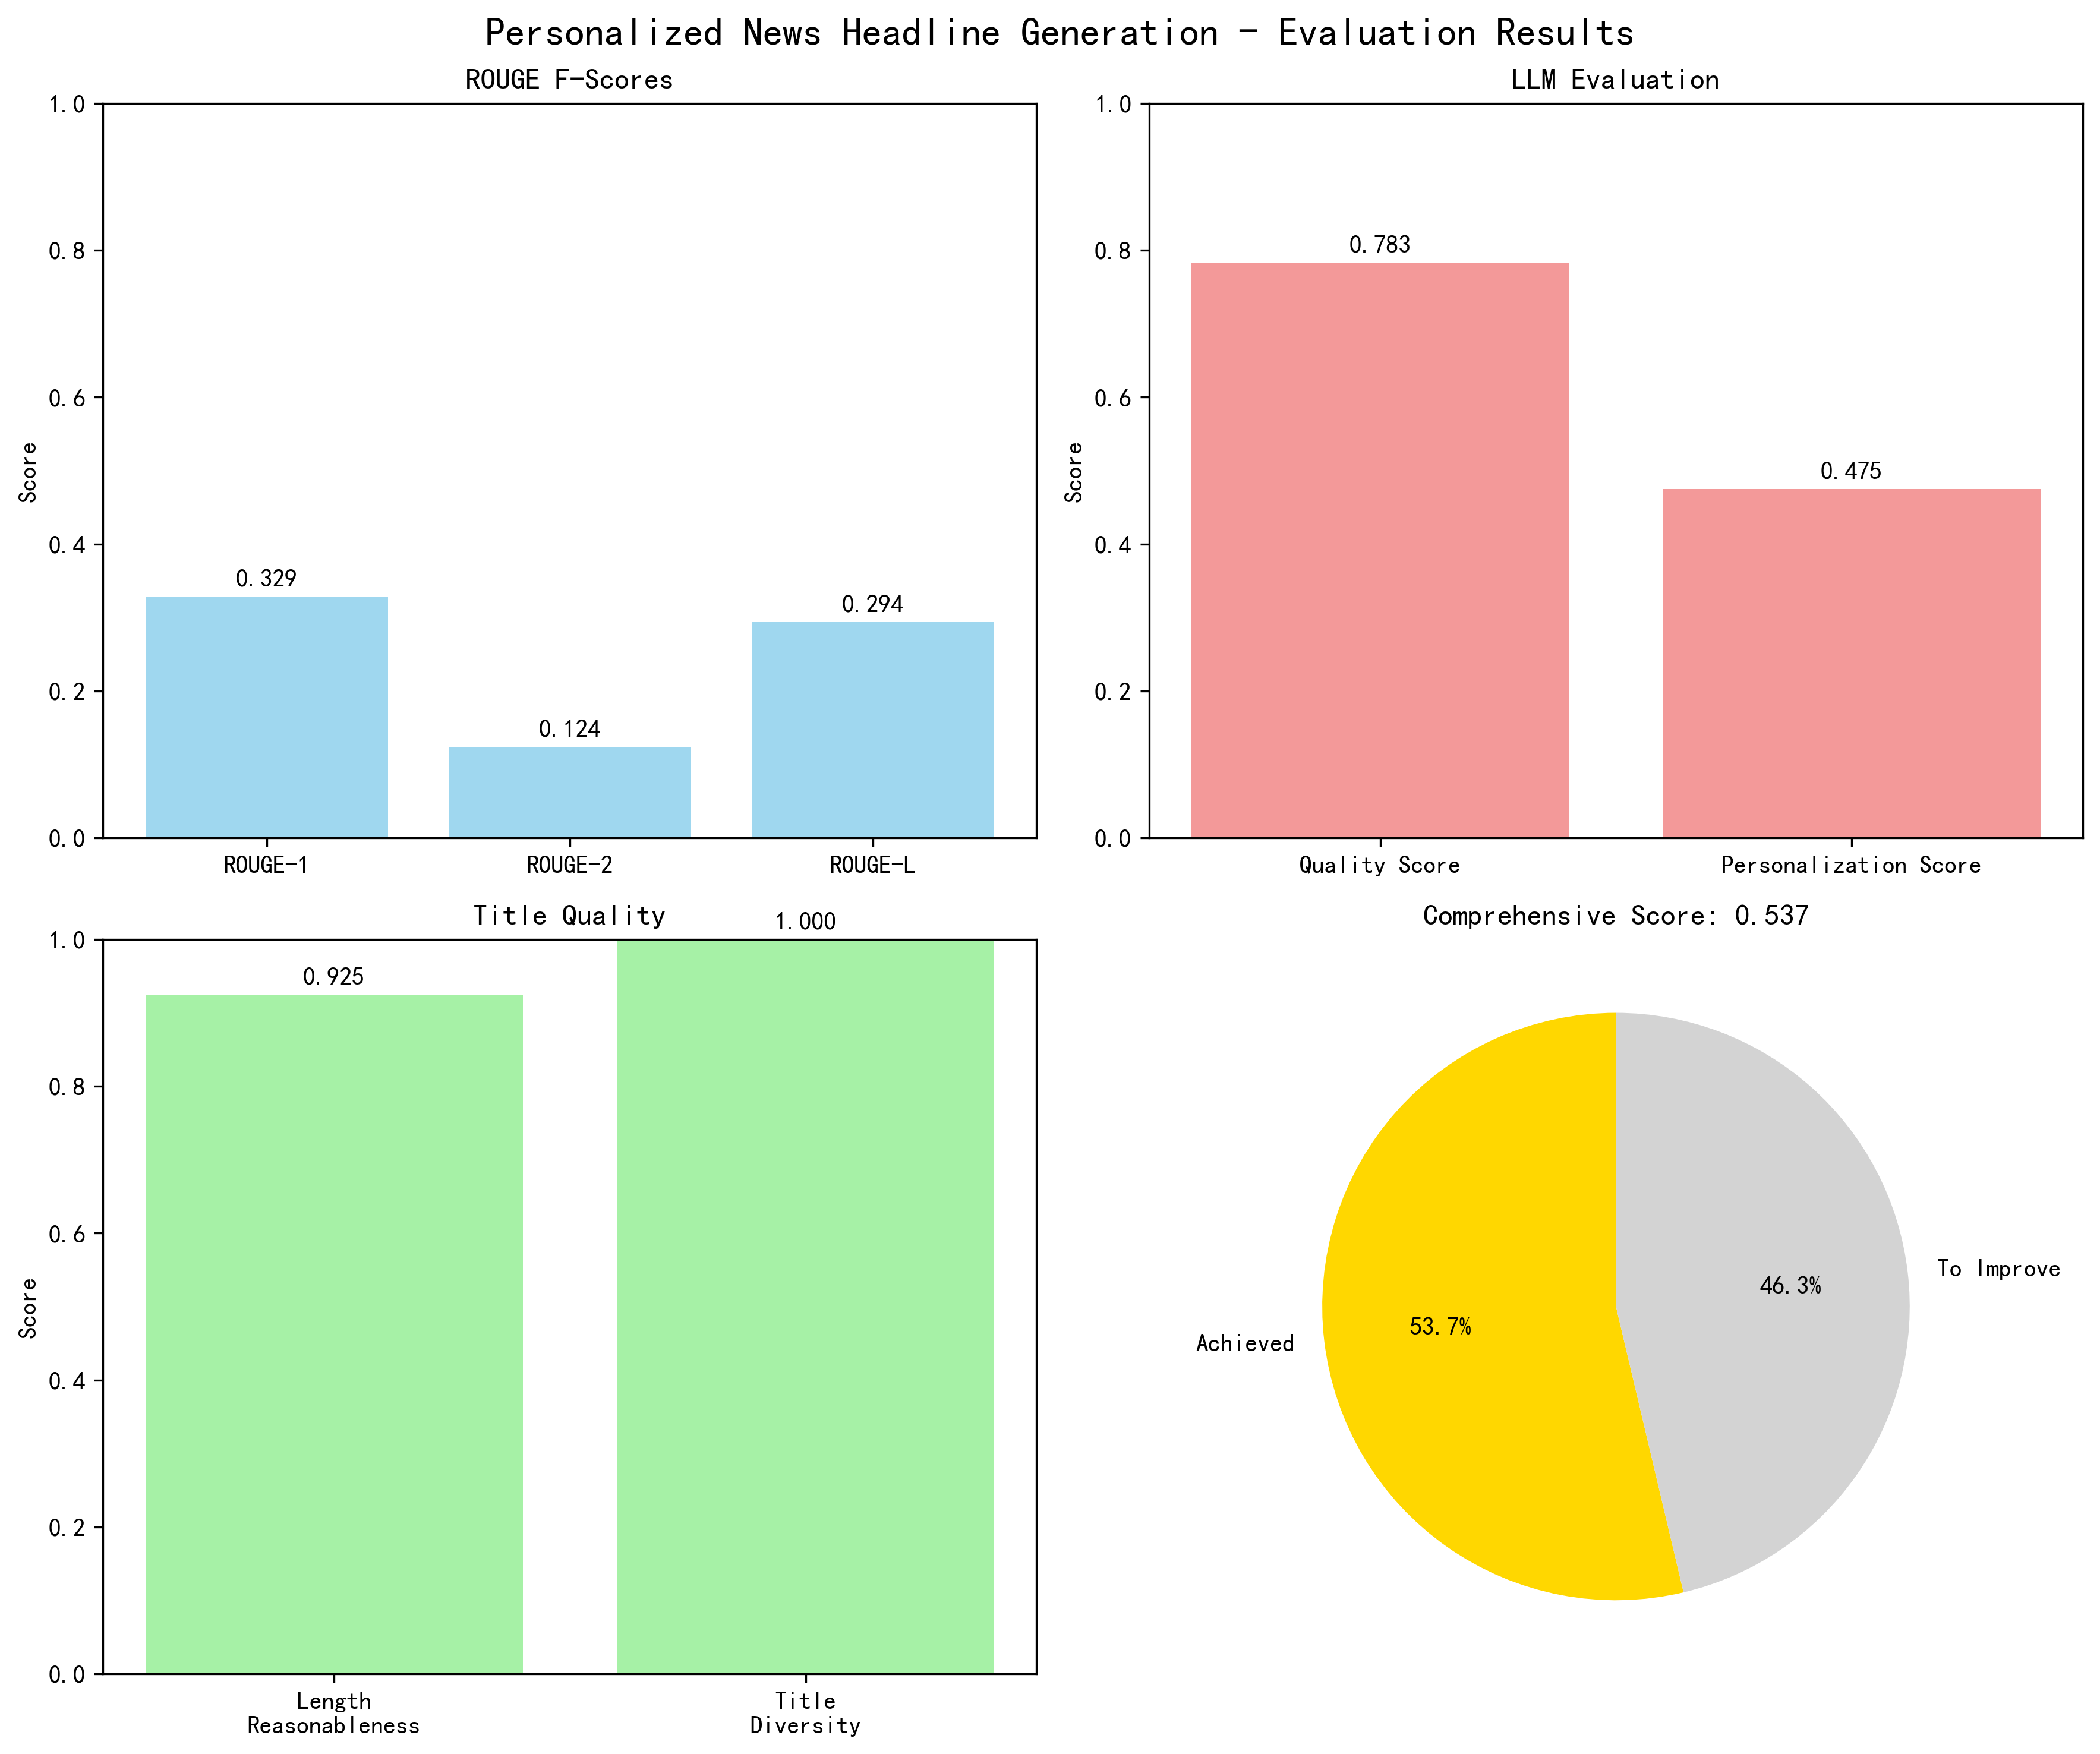
\includegraphics[width=\textwidth]{fig/evaluation_chart_20250622_212308.png}   
  \caption{提示词工程方法评估结果}\label{fig:prompt_evaluation}
\end{figure}

\subsection{实验结果}
基于ChavAPI平台的大语言模型调用,本项目完成了测试样本的个性化标题生成实验。实验采用DeepSeek-Chat-V3模型作为主要生成模型和评估模型。

从ROUGE自动评估结果来看,系统取得了较为理想的性能表现:\textbf{ROUGE-1 F值达到0.3286,ROUGE-2 F值为0.1238,ROUGE-L F值为0.2938}。这些指标明显高于基线方法性能表现的峰值,表明生成的个性化标题与参考标题在词汇覆盖率和语言结构方面具有较好的相似性。

LLM智能评估也对标题的生成结果做出了客观公正的评价。在质量评估方面,系统获得了0.783的综合质量分数(满分1.0),等效于10分制下的7.83分,表明生成的标题在准确性、吸引力、清晰度等维度都达到了较高水平。个性化评估方面,兴趣匹配度达到0.70,类别相关性为0.5625,历史一致性为0.575,体现了系统在理解用户偏好和生成相关内容方面的能力。

从具体生成案例来看,系统能够根据用户的兴趣领域调整标题的表达方式和重点。例如,对于关注法律政治类新闻的用户,系统生成的标题"High-Stakes Legal Battle Erupts Over Trump's Rollback of Obama-Era Pollution Rules"突出了"法律战"和"高风险"等关键词;对于体育爱好者,标题"Verlander Scolded by MLB Over Ball-Tampering Claims Ahead of All-Star Game"则强调了具体的球员和联盟动态。这些案例展现了提示词工程在个性化内容生成方面的灵活性和精确性。

综合评分方面,系统的最终得分为0.5370(满分1.0),其中LLM质量评估贡献最大(权重30\%,得分0.783),个性化效果评估也表现良好(权重25\%,得分0.475)。这一结果验证了提示词工程方法在平衡内容质量和个性化效果方面的有效性。

\section{基线方法与提示词工程对比分析}
通过对PENS基线方法和提示词工程方法的深入分析与实验验证,可以从技术架构、实现复杂度、性能表现、实用性等多个维度进行综合对比。

\textbf{技术架构对比:}基线方法采用传统的深度学习流水线,包含数据预处理、用户编码器训练、个性化生成器预训练与微调等多个阶段,整个架构较为复杂但逻辑清晰。提示词工程方法则采用"数据预处理+提示词设计+LLM调用"的简化架构,避免了复杂的模型训练过程,但对提示词设计的质量要求更高。从技术先进性角度,基线方法体现了序列到序列生成和注意力机制的经典应用,而提示词工程方法则代表了大语言模型时代的新兴技术路线。

\textbf{实现复杂度对比:}基线方法的环境搭建相对复杂,需要配置CUDA环境、管理GPU显存、处理PyTorch版本兼容性等问题,对硬件要求较高。训练过程涉及大量的超参数调节,包括学习率调度、批次大小优化、早停策略等,需要较强的深度学习背景知识。提示词工程方法的实现门槛明显更低,主要依赖标准的Python环境和API调用,无需GPU硬件支持,对技术背景要求相对较低。然而,提示词设计本身是一门艺术,需要对任务领域有深入理解。

\textbf{性能表现对比:}从ROUGE评估指标来看,基线方法在训练收敛后能够达到相对较高的词汇重叠度,这主要得益于端到端的训练优化和大量训练数据的学习。提示词工程方法的ROUGE分数明显提高(ROUGE-1: 0.3286 vs 基线方法峰值0.2419),在个性化效果方面表现也更为突出。基线方法的个性化主要依赖用户编码器学习到的隐式表示,而提示词工程方法能够更直观地融合用户兴趣信息,在兴趣匹配度等维度上展现优势。

\textbf{可扩展性与泛化性对比:}基线方法一旦训练完成,模型参数相对固定,扩展到新领域或适应新需求需要重新训练,成本较高。提示词工程方法具有更强的灵活性,可以通过调整提示词模板快速适应不同的任务需求,支持多语言、多领域的扩展。此外,随着大语言模型能力的不断提升,提示词工程方法能够持续受益于基座模型的改进,而无需额外的训练成本。

\textbf{资源消耗与成本对比:}基线方法的训练阶段需要大量的计算资源,包括GPU训练时间、电力消耗等,但推理阶段相对高效。提示词工程方法将计算负担转移到了云端API服务,单次调用成本较低,但对于大规模应用可能面临API费用累积的问题。从研究与开发的角度,提示词工程方法能够更快地进行原型验证和迭代优化。

\textbf{可解释性与可控性对比:}基线方法的神经网络结构具有一定的"黑盒"特性,虽然可以通过注意力权重等方式进行一定程度的解释,但整体的决策过程较为隐晦。提示词工程方法的生成过程更加透明,用户可以直观地理解输入信息如何影响输出结果,便于调试和优化。在内容安全和合规性方面,提示词工程方法也更容易实现精确控制。

综合而言,两种方法各有优势,适用于不同的应用场景。基线方法更适合对性能要求极高、数据量充足、计算资源丰富的场景,如大型媒体平台的批量标题生成。提示词工程方法则更适合快速原型开发、跨领域应用、个性化要求较高的场景,特别是在大语言模型能力持续提升的当下,其发展前景更为广阔。从技术发展趋势来看,两种方法的融合应用可能是未来的重要方向,即利用深度学习方法进行用户表示学习,同时结合提示词工程实现灵活的内容生成,以兼顾性能表现和系统灵活性。

\section{小组分工}
朱首赫:基线方法的复现与改进、数据集内部结构研究与分析、报告文档1-2节撰写。

王荦璠:提示词工程方法设计与实现、ChavAPI平台搭建与优化、多维度评估体系构建、报告文档3-4节撰写。

\end{document}